\documentclass[sigconf]{acmart}
% =============================================================================
% Template setup -- participants normally do not edit this file.
% Author content belongs in main.tex; citations belong in main.bib.
% \documentclass lives in main.tex so Overleaf does not treat this file as root.
% (Reproduced from the organizers' template; unchanged.)
% =============================================================================

% --- Competition / non-ACM-submission friendly rights metadata -------------
\setcopyright{none}
\settopmatter{printacmref=false}
\acmConference[Kaggle Competition]{Filament Segmentation Challenge}{2026}{\href{https://www.kaggle.com/competitions/filament-segmentation-2026}{kaggle.com/competitions/filament-segmentation-2026}}
\acmBooktitle{Competition Report}
\acmDOI{}
\acmISBN{}

% --- Author guidance text --------------------------------------------------
% \guide{...} is gray italic while \guideStyletrue; omitted from the PDF if false.
% Flip the switch in main.tex after % =============================================================================
% Template setup -- participants normally do not edit this file.
% Author content belongs in main.tex; citations belong in main.bib.
% \documentclass lives in main.tex so Overleaf does not treat this file as root.
% (Reproduced from the organizers' template; unchanged.)
% =============================================================================

% --- Competition / non-ACM-submission friendly rights metadata -------------
\setcopyright{none}
\settopmatter{printacmref=false}
\acmConference[Kaggle Competition]{Filament Segmentation Challenge}{2026}{\href{https://www.kaggle.com/competitions/filament-segmentation-2026}{kaggle.com/competitions/filament-segmentation-2026}}
\acmBooktitle{Competition Report}
\acmDOI{}
\acmISBN{}

% --- Author guidance text --------------------------------------------------
% \guide{...} is gray italic while \guideStyletrue; omitted from the PDF if false.
% Flip the switch in main.tex after % =============================================================================
% Template setup -- participants normally do not edit this file.
% Author content belongs in main.tex; citations belong in main.bib.
% \documentclass lives in main.tex so Overleaf does not treat this file as root.
% (Reproduced from the organizers' template; unchanged.)
% =============================================================================

% --- Competition / non-ACM-submission friendly rights metadata -------------
\setcopyright{none}
\settopmatter{printacmref=false}
\acmConference[Kaggle Competition]{Filament Segmentation Challenge}{2026}{\href{https://www.kaggle.com/competitions/filament-segmentation-2026}{kaggle.com/competitions/filament-segmentation-2026}}
\acmBooktitle{Competition Report}
\acmDOI{}
\acmISBN{}

% --- Author guidance text --------------------------------------------------
% \guide{...} is gray italic while \guideStyletrue; omitted from the PDF if false.
% Flip the switch in main.tex after \input{preamble}.
%
% Do not use \guide{...} for \email{...}.
\usepackage{xcolor}
\newif\ifguideStyle
\guideStyletrue
\newcommand{\guide}[1]{%
  \ifguideStyle
    {\color{gray!65}\itshape #1}%
  \fi
}

% --- Math ------------------------------------------------------------------
% Do NOT load amssymb (or amsfonts): acmart already loads newtxmath, which
% defines the same symbols (e.g. \Bbbk) and causes a conflict on Overleaf.
% amsmath is already provided by acmart; mathtools extends it.
\usepackage{mathtools}

% --- Figures ---------------------------------------------------------------
% graphicx is already loaded by acmart
\usepackage{subcaption}

% --- Tables ----------------------------------------------------------------
% booktabs is already loaded by acmart
\usepackage{tabularx}
\usepackage{multirow}

% --- Bibliography style is set in main.tex (ACM-Reference-Format) ----------
.
%
% Do not use \guide{...} for \email{...}.
\usepackage{xcolor}
\newif\ifguideStyle
\guideStyletrue
\newcommand{\guide}[1]{%
  \ifguideStyle
    {\color{gray!65}\itshape #1}%
  \fi
}

% --- Math ------------------------------------------------------------------
% Do NOT load amssymb (or amsfonts): acmart already loads newtxmath, which
% defines the same symbols (e.g. \Bbbk) and causes a conflict on Overleaf.
% amsmath is already provided by acmart; mathtools extends it.
\usepackage{mathtools}

% --- Figures ---------------------------------------------------------------
% graphicx is already loaded by acmart
\usepackage{subcaption}

% --- Tables ----------------------------------------------------------------
% booktabs is already loaded by acmart
\usepackage{tabularx}
\usepackage{multirow}

% --- Bibliography style is set in main.tex (ACM-Reference-Format) ----------
.
%
% Do not use \guide{...} for \email{...}.
\usepackage{xcolor}
\newif\ifguideStyle
\guideStyletrue
\newcommand{\guide}[1]{%
  \ifguideStyle
    {\color{gray!65}\itshape #1}%
  \fi
}

% --- Math ------------------------------------------------------------------
% Do NOT load amssymb (or amsfonts): acmart already loads newtxmath, which
% defines the same symbols (e.g. \Bbbk) and causes a conflict on Overleaf.
% amsmath is already provided by acmart; mathtools extends it.
\usepackage{mathtools}

% --- Figures ---------------------------------------------------------------
% graphicx is already loaded by acmart
\usepackage{subcaption}

% --- Tables ----------------------------------------------------------------
% booktabs is already loaded by acmart
\usepackage{tabularx}
\usepackage{multirow}

% --- Bibliography style is set in main.tex (ACM-Reference-Format) ----------

\setlength{\emergencystretch}{3em}
\usepackage{tikz}
\usetikzlibrary{positioning,arrows.meta}

% Guide styling: \guideStyletrue = show gray italic hints; \guideStylefalse = omit them
% \guideStyletrue
\guideStylefalse

\begin{document}

\title[Two-Stage Solar Filament Segmentation]{Two-Stage Solar Filament Instance Segmentation: A U-Net Ensemble, a Crop Refiner and a Break-Even Instance Scorer}
\subtitle{A Solution to the Solar Filament Segmentation Challenge 2026} % DO NOT CHANGE

\author{Abu Kayyisah Basyid}
\email{basyid238@gmail.com}

\begin{abstract}
    This report describes our solution to the Solar Filament Segmentation Challenge~2026, a Kaggle competition on automatic segmentation of solar filaments in GONG H-$\alpha$ observations.
    A five-fold ResNet34 U-Net ensemble with flip test-time augmentation proposes candidate instances; a crop-level refiner redraws each candidate from a box-shaped seed; a near-limb filter and a gradient-boosted instance scorer then drop instances that are unlikely to pay under the panoptic-quality (PQ) formula. The pipeline reaches PQ~0.443 on a 50-image hold-out never used for training or model selection, 0.409 out of fold on the 657 pool images (single models) and 0.37 on the public leaderboard; the mean Dice of the union masks is 0.66 on the hold-out. Two annotators agree with each other at only PQ~0.34, and most further ideas we tried (including multi-scale test-time augmentation and patch re-sampling) were indistinguishable from zero or harmful. The scorer raises PQ but lowers Dice, so we prepared two thresholds. Our own EfficientNetV2-S stage-A, trained on the same folds, reaches 0.432 out of fold and 0.38 on the public leaderboard, but it failed our pre-registered hold-out check (0.431 against 0.443); we nevertheless chose it as the final submission, a departure from that rule that we state openly. We use only the competition's own data.
\end{abstract}

\maketitle

% =============================================================================
%                                INTRODUCTION
% =============================================================================
\section{Introduction}
    This report goes over the details of our submitted solution to the Solar Filament Segmentation Challenge~2026 \cite{filament-segmentation-2026}, organized by the Earth-Space AI Research (ESAIR) Lab\footnote{\href{https://www.esairlab.com/home}{www.esairlab.com/}}, which uses the MAGFiLO dataset \cite{ahmadzadeh2024dataset}.
    We describe a fully supervised, two-stage pipeline built only on the competition's data. With 50 hold-out images most differences between design choices are smaller than the sampling error, so we also score 657 images out of fold and report each difference with a paired bootstrap interval.

% =============================================================================
%                                METHODOLOGY
% =============================================================================
\section{Methodology}\label{sec:methodology}

\subsection{Data and splits}
We use the 707 annotated training images ($2048{\times}2048$) and the 180 test images. Each training image carries one to three annotator passes (411, 145 and 151 images); a pass is an independent set of instance polygons. A fixed hold-out of 50 images (seed 1234) is excluded from every training fold, from checkpoint selection and from the refiner's training. The remaining 657 images form five folds (about 526 images for training, 131 for choosing a checkpoint). ``Out of fold'' means that an image is scored by the fold model that did not train on it.

\begin{figure*}[t]
\centering
\begin{tikzpicture}[
  node distance=3.6mm, every node/.style={font=\scriptsize},
  box/.style={draw, rounded corners=2pt, align=center, inner sep=2.6pt, minimum height=1.0cm, fill=blue!6},
  arr/.style={-{Stealth[length=1.8mm]}, thick}]
  \node[box, fill=gray!12] (img) {H-$\alpha$ image\\$2048^2$};
  \node[box, right=of img] (a) {Stage-A: 5 U-Nets\\(ResNet34) $\times$ 4 flips\\$\Rightarrow$ probability map};
  \node[box, right=of a] (c) {Candidates: $p{>}0.4$,\\area $400$--$40000$,\\mean $p \ge 0.7$};
  \node[box, right=of c] (r) {Crop refiner (U-Net)\\input: image, CLAHE,\\padded-box seed};
  \node[box, right=of r] (l) {Near-limb filter\\centroid $>0.88R$\\dropped};
  \node[box, right=of l] (s) {Instance scorer\\(LightGBM, 36 feat.)\\drop if $<\tau$};
  \node[box, right=of s, fill=green!8] (o) {One mask per\\instance (RLE)};
  \draw[arr] (img) -- (a); \draw[arr] (a) -- (c); \draw[arr] (c) -- (r); \draw[arr] (r) -- (l); \draw[arr] (l) -- (s); \draw[arr] (s) -- (o);
\end{tikzpicture}
\caption{End-to-end pipeline. Everything is inference-only after training. $R$ is the solar-disk radius; $\tau$ is the scorer threshold (Section~\ref{sec:scorer}).}
\label{fig:pipeline}
\end{figure*}

\subsection{Pipeline}
Figure~\ref{fig:pipeline} summarises the pipeline.
\paragraph{Stage-A.} Five U-Nets \cite{ronneberger2015unet} with ImageNet-initialised ResNet34 encoders \cite{he2016resnet}, one per fold, are trained for 30 epochs of 220 steps (batch 8, 512-px patches, 75\% centred on filaments) with a Tversky loss ($\alpha{=}0.3$, $\beta{=}0.7$) \cite{salehi2017tversky} plus binary cross-entropy, AdamW \cite{loshchilov2019decoupled} and a one-cycle schedule \cite{smith2017superconvergence} peaking at $10^{-4}$. The target is the pixel union of all annotator passes. At inference the probabilities of 5 models $\times$ 4 flips are averaged over 512-px windows with stride 384.

\paragraph{Candidates.} We threshold at 0.4, close with a $3{\times}3$ ellipse, take 8-connected components and keep those with area 400--40000 px and mean probability $\ge 0.7$.

\paragraph{Crop refiner.} For each candidate a square crop (1.5$\times$ the longest box side, at least 96 px) is resized to $512^2$ and fed as three channels: the crop, its CLAHE version \cite{zuiderveld1994clahe} and a seed, the bounding box padded by 40\%. A ResNet34 U-Net \cite{iakubovskii2019smp} predicts the mask (threshold 0.5). It is trained for 13 epochs on 6,474 crops (every annotator instance is one sample) with the loss $0.45\,\text{BCE}+0.55\,\text{soft Dice}$; the seed box is jittered so the network cannot copy it.

\paragraph{Near-limb filter.} The disk is estimated per image (Otsu threshold, largest component); instances whose centroid lies beyond $0.88R$ are dropped. The threshold was chosen out of fold (+0.0065 PQ).

\paragraph{Instance scorer.}\label{sec:scorer} Under PQ, keeping an instance adds its matched IoU to the numerator and $0.5$ to the denominator in every pass, so it pays only if its expected matched IoU exceeds PQ$/2$. A LightGBM \cite{ke2017lightgbm} regressor on 36 inference-time features (stage-A probability statistics, shape, contrast, disk position, neighbourhood), fitted on the 4,694 out-of-fold instances, predicts that quantity; instances below $\tau{=}0.1972$ are dropped. This is half of the near-limb out-of-fold PQ ($0.3944/2$), fixed in advance from the pre-scorer PQ and not tuned. Cross-validated by image the scorer reaches AUC 0.784 and removes 14.5\% of the instances on the test set.

\begin{figure*}[t]
\centering
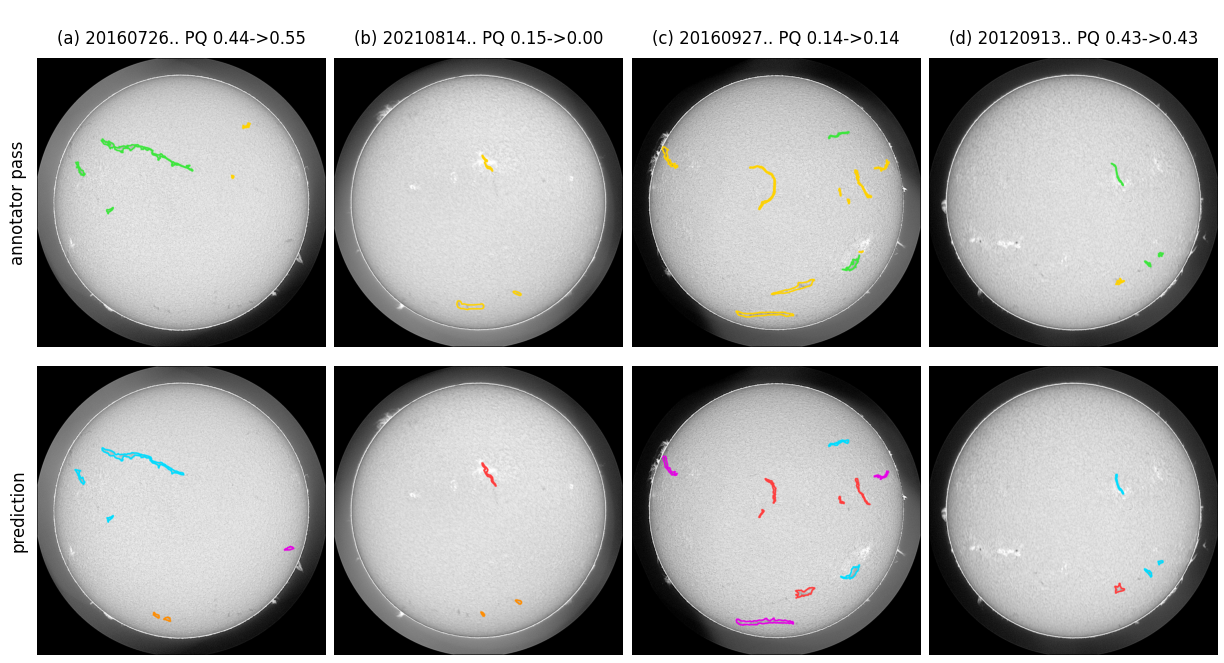
\includegraphics[width=0.93\textwidth]{fig_cases.png}
\caption{Four hold-out images chosen by a rule fixed beforehand: (a) the image the scorer helps most, (b) hurts most, (c) the lowest PQ among images with $\ge$4 annotated filaments (the next one after (b)), (d) the median PQ. The annotator pass with most instances is shown. Top: annotated filaments, matched by a kept prediction (green) or missed (yellow). Bottom: kept predictions, matched (cyan) or unmatched (red); candidates dropped by the instance scorer (orange) or by the near-limb filter (magenta). Titles: per-image PQ without $\to$ with the scorer.}
\label{fig:examples}
\end{figure*}

% =============================================================================
%                                EVALUATION
% =============================================================================
\section{Evaluation}\label{sec:evaluation}

\subsection{Protocol}
We use the official panoptic quality \cite{kirillov2019panoptic}, $\text{PQ}=\sum_{TP}\text{IoU}/(|TP|+\tfrac12|FP|+\tfrac12|FN|)$ with a match at $\text{IoU}>0.5$, computed against every annotator pass and pooled. Uncertainty is a bootstrap over images (4000 resamples); the hold-out standard error of PQ is 0.017, that of the 657 out-of-fold images 0.005. The other rubric quantities follow the organizers' self-evaluation notebook: pairwise IoU and Dice between ground-truth and predicted instances of one annotator-image (pairs with a score above 0), and the one-to-many and many-to-one counts (partners with IoU above 0). The configuration of the mean-Dice scorer is not stated; we report the Dice of the union masks (foreground) per image.

\begin{table}[t]
\centering
\caption{Progression. Hold-out: 50 images, 5-model ensemble. OOF: 657 images, each scored by a single model that did not train on it. $^\dagger$proxy metric.}
\label{tab:main}
\small
\begin{tabular}{@{}lccc@{}}
\toprule
Configuration & Hold-out PQ & OOF PQ & LB\\
\midrule
5-fold ensemble, no TTA$^\dagger$ & 0.3754 & -- & 0.33\\
\quad + flip TTA & 0.4151 & 0.367 & --\\
\quad + crop refiner & 0.4325 & 0.388 & 0.36\\
\quad + near-limb filter & 0.4383 & 0.394 & --\\
\quad + instance scorer (released) & 0.4427 & 0.409 & 0.37\\
\quad + own EfficientNetV2-S stage-A (final) & 0.4309 & 0.432 & \textbf{0.38}\\
\bottomrule
\end{tabular}
\end{table}

\subsection{Results}
The final pipeline reaches PQ 0.4427 on the hold-out, 0.409 out of fold and 0.37 on the public leaderboard (rank 167 of 806 on 1 October; the scoreboard shows about half of the test images). The refiner adds $+0.0177$ on the hold-out (its leaderboard gain is not measured separately); the scorer adds $+0.0144$ out of fold (CI95 $+0.011$ to $+0.018$), $+0.0043$ on the hold-out (not significant on 50 images) and $+0.01$ on the leaderboard. Table~\ref{tab:rubric} gives the quantities of the rubric other than PQ: over-merging is rare (2\% of predictions touch two or more annotated filaments) and splitting is small (3\% of annotated filaments); the dominant relation is a miss.

\paragraph{Our own EfficientNetV2-S stage-A.} After the released pipeline was fixed, we trained a U-Net with an EfficientNetV2-S encoder on the same five folds, with our own code and a recipe described on a public model card (10,500 steps per fold, soft multi-annotator target; about 2.15 GPU-hours per fold on a T4). With loose candidates, the near-limb filter and a scorer refit on each model set, it scores 0.432 out of fold against 0.409 for the released pipeline ($+0.023$, CI95 $+0.017$ to $+0.029$). On the 50 hold-out images its five-model ensemble scores 0.431 against 0.443, and this difference is inside the hold-out standard error; because the pre-registered rule required both conditions, the model was not adopted. Its public score is 0.38. We chose it as the final submission after this check, against that rule; the decision is the authors' and is reported as such. For comparison, a public third-party stage-A (CC BY 4.0, evaluated out of fold with our post-processing) reached 0.455; it is not part of any submission.

\begin{table}[t]
\centering
\caption{Rubric quantities of the final pipeline (union-mask Dice per image; relations by overlap $>0$).}
\label{tab:rubric}
\small
\begin{tabular}{@{}lcc@{}}
\toprule
 & OOF (657) & Hold-out (50)\\
\midrule
PQ & 0.409 & 0.443\\
Mean Dice (union masks) & 0.624 & 0.664\\
Pairwise IoU / Dice (pairs $>0$) & 0.578 / 0.712 & 0.593 / 0.725\\
Ground truth with no prediction (1:0) & 26.8\% & 24.4\%\\
Predictions with no ground truth (0:1) & 12.3\% & 9.8\%\\
Ground truth split in $\ge$2 (1:n) & 3.4\% & 3.7\%\\
Predictions merging $\ge$2 (n:1) & 2.4\% & 1.9\%\\
\bottomrule
\end{tabular}
\end{table}

\subsection{Two thresholds: PQ versus Dice}
The scorer trades Dice for PQ: without it the out-of-fold Dice is 0.633 and with it 0.624 (paired $-0.0084$, CI95 $-0.014$ to $-0.004$; hold-out $-0.0123$), because the dropped instances raise the share of unmatched annotated filaments from 20.6\% to 26.8\%. The rubric weights of Dice and PQ are not published, so we prepared two configurations that differ only in $\tau$ (Table~\ref{tab:tau}); both are reproducible from the same repository. A sweep of $\tau$ on the out-of-fold images shows that Dice drops mainly between $\tau{=}0.15$ and $0.25$; 0.15 was selected on the same images and has no independent confirmation.

\begin{table}[t]
\centering
\caption{Scorer threshold: PQ / mean Dice, and the paired difference (0.15 minus released), with CI95.}
\label{tab:tau}
\small
\begin{tabular}{@{}lcc@{}}
\toprule
 & OOF (657) & Hold-out (50)\\
\midrule
$\tau{=}0.1972$ (released) & 0.4089 / 0.624 & 0.4427 / 0.664\\
$\tau{=}0.15$ (balanced) & 0.4063 / 0.631 & 0.4418 / 0.668\\
$\Delta$PQ & $-0.0027$ [$-0.005,-0.001$] & $-0.0009$ [$-0.009,+0.006$]\\
$\Delta$Dice & $+0.0072$ [$+0.004,+0.011$] & $+0.0046$ [$+0.001,+0.008$]\\
\bottomrule
\end{tabular}
\end{table}

\subsection{Negative results}
Table~\ref{tab:neg} lists what did not help. Two deserve a note. Averaging the maps of scales 0.75, 1.0 and 1.25 gains $+0.0117$ out of fold for single models (CI95 $+0.007$ to $+0.017$) but loses $0.0114$ for the five-model ensemble on the hold-out, which already averages 20 predictions; the test run was therefore not made. Re-sampling the stage-A training patches in every epoch (the production sampler repeats 1,760 distinct patches) lowers the out-of-fold PQ by $0.020$ in all five folds because the retrained models produce many more false positives under the fixed candidate thresholds.

\begin{table}[t]
\centering
\caption{Ideas that did not help (change in PQ; paired, out of fold unless noted).}
\label{tab:neg}
\small
\begin{tabular}{@{}p{5.7cm}r@{}}
\toprule
Idea & $\Delta$PQ\\
\midrule
Per-epoch re-sampling of stage-A patches (5 folds) & $-0.0202$\\
Multi-scale TTA, 5-model ensemble (hold-out) & $-0.0114$\\
EMA weights, ensemble (hold-out) & $-0.0101$\\
Consensus ($\ge$2-pass) target, 5 folds & $+0.0023$\\
Hard-negative training of the refiner & $+0.0006$\\
Ensemble with a public Mask R-CNN & $+0.0028$\\
Per-instance mask-variant selection (oracle $+0.0223$) & $-0.0013$\\
Refiner features in the scorer & $-0.0005$\\
Re-tuned thresholds for single-pass images & $+0.0003$\\
\bottomrule
\end{tabular}
\end{table}

\subsection{Error analysis and uncertainty}
Figure~\ref{fig:examples} shows the filters at work. In (a) the scorer removes two small candidates and the three kept predictions match three of five annotated filaments (PQ 0.44$\to$0.55). In (b) it removes two candidates, one of which matched an annotated filament, and keeps one that matches nothing (PQ 0.15$\to$0.00): its expected-IoU estimate fails on faint structures. In (c) the near-limb filter removes three candidates close to the limb, where annotated filaments also lie, and only 2 of 11 annotated filaments are matched. Many unmatched predictions are short dark structures, some of which may be real but unannotated (the challenge forum reports missing annotations). Of the 450 hold-out errors of the refiner-stage pipeline, 54\% are near-misses (a prediction overlaps a filament with $\text{IoU}\le0.5$). Treating one annotator pass as a prediction of another with the same rules gives only PQ~0.34 (mean matched IoU 0.63; 0.14\% of matched pairs reach IoU 0.85), so the ceiling set by the labels is low (Fig.~\ref{fig:unc}); an oracle that removes exactly the instances below break-even would add $+0.074$, of which the scorer captures $+0.014$.

The out-of-fold estimate of this recipe (about 0.41 for an ensemble) is above the leaderboard (0.37). Using only stored predictions we could not attribute the gap to the test images: a classifier separating test from out-of-fold instances on 26 geometry and image features reaches AUC 0.51, inside the range of 20 label permutations (0.44--0.56), and re-weighting the out-of-fold images to the test mixture moves PQ from 0.409 to 0.414, away from the leaderboard. What remains are properties invisible to the predictions (annotator style or number of passes in the test labels) and the noise of a score computed on part of 180 images.

\begin{figure}[t]
\centering
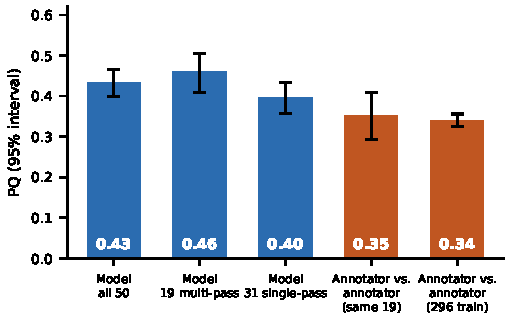
\includegraphics[width=\columnwidth]{fig_uncertainty.pdf}
\caption{PQ with 95\% bootstrap intervals (refiner-stage pipeline): our model (blue) versus annotators scored against each other (orange).}
\label{fig:unc}
\end{figure}

\subsection{Strengths, weaknesses, and possible improvements}
\textbf{Strengths.} The pipeline is simple, reproducible, tested (unit tests for the metric, candidate extraction, filters and scorer) and needs about 3 minutes per image on a 4-core CPU; the break-even rule gives the scorer without tuning. \textbf{Weaknesses.} The hold-out cannot resolve small gains and several thresholds were tuned on it; the scorer's hold-out gain is not significant; the gap to the leaderboard is unexplained; the scorer lowers Dice. \textbf{Improvements.} A stage-A trained with more diverse patches needs thresholds and a refiner refitted to its maps; models that see more context than a 512-px window and a second ensemble were not tried for lack of expected gain per unit of the shared GPU budget.

\subsection{Data compliance and reproducibility}
Only the competition's training images and annotations were used. The public MAGFiLO release is reported by participants to contain annotations of the test images; we neither downloaded nor consulted it, and used no test labels or third-party submission files. To understand the leaderboard we decoded one public notebook that embeds a pre-computed submission and computed descriptive statistics only; it was never used for training, tuning, selection or evaluation. Code, tests and an end-to-end notebook are at \url{https://github.com/Alphine/filament}; the trained weights of both stage-A models, the refiner and the scorer (Apache-2.0, with SHA256 checksums) are published as a Kaggle dataset at \url{https://www.kaggle.com/datasets/abukayyisahbasyid/solar-filament-segmentation-2026-weights}. The weights of the public third-party model are neither used in any submission nor redistributed. The code and this report were developed with an AI coding assistant under the author's direction.

% =============================================================================
%                              ACKNOWLEDGMENT
% =============================================================================
\section{Acknowledgment}\label{sec:acknowledgment}
    % Do not change
    The organization of the Filament Segmentation Challenge 2026 is partially supported by the U.S. National Science Foundation (NSF) under Grant No. 2209912 and 2433781, directorate for Computer and Information Science and Engineering (CSE), and Office of Advanced Cyberinfrastructure (OAC), and Grant No. 2511630, AST Division Of Astronomical Sciences and MPS Directorate for Mathematical and Physical Sciences.

    The Filament Segmentation Challenge 2026 is sponsored by the U.S. National Science Foundation (NSF) National Solar Observatory (NSO).

    This work utilizes GONG data obtained by the NSO Integrated Synoptic Program, managed by the National Solar Observatory, which is operated by the Association of Universities for Research in Astronomy (AURA), Inc. under a cooperative agreement with the National Science Foundation and with contribution from the National Oceanic and Atmospheric Administration. The GONG network of instruments is hosted by the Big Bear Solar Observatory, High Altitude Observatory, Learmonth Solar Observatory, Udaipur Solar Observatory, Instituto de Astrofísica de Canarias, and Cerro Tololo Interamerican Observatory.

\bibliographystyle{ACM-Reference-Format}
\bibliography{main}

\end{document}
